% Options for packages loaded elsewhere
% Options for packages loaded elsewhere
\PassOptionsToPackage{unicode}{hyperref}
\PassOptionsToPackage{hyphens}{url}
\PassOptionsToPackage{dvipsnames,svgnames,x11names}{xcolor}
%
\documentclass[
  russian,
]{article}
\usepackage{xcolor}
\usepackage[top=20mm,left=20mm,right=20mm,bottom=20mm]{geometry}
\usepackage{amsmath,amssymb}
\setcounter{secnumdepth}{5}
\usepackage{iftex}
\ifPDFTeX
  \usepackage[T1]{fontenc}
  \usepackage[utf8]{inputenc}
  \usepackage{textcomp} % provide euro and other symbols
\else % if luatex or xetex
  \usepackage{unicode-math} % this also loads fontspec
  \defaultfontfeatures{Scale=MatchLowercase}
  \defaultfontfeatures[\rmfamily]{Ligatures=TeX,Scale=1}
\fi
\usepackage{lmodern}
\ifPDFTeX\else
  % xetex/luatex font selection
  \setmainfont[]{Times New Roman}
  \setsansfont[]{Arial}
  \setmonofont[]{Courier New}
\fi
% Use upquote if available, for straight quotes in verbatim environments
\IfFileExists{upquote.sty}{\usepackage{upquote}}{}
\IfFileExists{microtype.sty}{% use microtype if available
  \usepackage[]{microtype}
  \UseMicrotypeSet[protrusion]{basicmath} % disable protrusion for tt fonts
}{}
\makeatletter
\@ifundefined{KOMAClassName}{% if non-KOMA class
  \IfFileExists{parskip.sty}{%
    \usepackage{parskip}
  }{% else
    \setlength{\parindent}{0pt}
    \setlength{\parskip}{6pt plus 2pt minus 1pt}}
}{% if KOMA class
  \KOMAoptions{parskip=half}}
\makeatother
% Make \paragraph and \subparagraph free-standing
\makeatletter
\ifx\paragraph\undefined\else
  \let\oldparagraph\paragraph
  \renewcommand{\paragraph}{
    \@ifstar
      \xxxParagraphStar
      \xxxParagraphNoStar
  }
  \newcommand{\xxxParagraphStar}[1]{\oldparagraph*{#1}\mbox{}}
  \newcommand{\xxxParagraphNoStar}[1]{\oldparagraph{#1}\mbox{}}
\fi
\ifx\subparagraph\undefined\else
  \let\oldsubparagraph\subparagraph
  \renewcommand{\subparagraph}{
    \@ifstar
      \xxxSubParagraphStar
      \xxxSubParagraphNoStar
  }
  \newcommand{\xxxSubParagraphStar}[1]{\oldsubparagraph*{#1}\mbox{}}
  \newcommand{\xxxSubParagraphNoStar}[1]{\oldsubparagraph{#1}\mbox{}}
\fi
\makeatother


\usepackage{longtable,booktabs,array}
\newcounter{none} % for unnumbered tables
\usepackage{calc} % for calculating minipage widths
% Correct order of tables after \paragraph or \subparagraph
\usepackage{etoolbox}
\makeatletter
\patchcmd\longtable{\par}{\if@noskipsec\mbox{}\fi\par}{}{}
\makeatother
% Allow footnotes in longtable head/foot
\IfFileExists{footnotehyper.sty}{\usepackage{footnotehyper}}{\usepackage{footnote}}
\makesavenoteenv{longtable}
\usepackage{graphicx}
\makeatletter
\newsavebox\pandoc@box
\newcommand*\pandocbounded[1]{% scales image to fit in text height/width
  \sbox\pandoc@box{#1}%
  \Gscale@div\@tempa{\textheight}{\dimexpr\ht\pandoc@box+\dp\pandoc@box\relax}%
  \Gscale@div\@tempb{\linewidth}{\wd\pandoc@box}%
  \ifdim\@tempb\p@<\@tempa\p@\let\@tempa\@tempb\fi% select the smaller of both
  \ifdim\@tempa\p@<\p@\scalebox{\@tempa}{\usebox\pandoc@box}%
  \else\usebox{\pandoc@box}%
  \fi%
}
% Set default figure placement to htbp
\def\fps@figure{htbp}
\makeatother



\ifLuaTeX
\usepackage[bidi=basic,shorthands=off,provide=*]{babel}
\else
\usepackage[bidi=default,shorthands=off,provide=*]{babel}
\fi
\ifPDFTeX
\else
\babelfont{rm}[]{Times New Roman}
\fi
\ifLuaTeX
  \usepackage{selnolig} % disable illegal ligatures
\fi


\setlength{\emergencystretch}{3em} % prevent overfull lines

\providecommand{\tightlist}{%
  \setlength{\itemsep}{0pt}\setlength{\parskip}{0pt}}



 


\makeatletter
\@ifpackageloaded{tcolorbox}{}{\usepackage[skins,breakable]{tcolorbox}}
\@ifpackageloaded{fontawesome5}{}{\usepackage{fontawesome5}}
\definecolor{quarto-callout-color}{HTML}{909090}
\definecolor{quarto-callout-note-color}{HTML}{0758E5}
\definecolor{quarto-callout-important-color}{HTML}{CC1914}
\definecolor{quarto-callout-warning-color}{HTML}{EB9113}
\definecolor{quarto-callout-tip-color}{HTML}{00A047}
\definecolor{quarto-callout-caution-color}{HTML}{FC5300}
\definecolor{quarto-callout-color-frame}{HTML}{acacac}
\definecolor{quarto-callout-note-color-frame}{HTML}{4582ec}
\definecolor{quarto-callout-important-color-frame}{HTML}{d9534f}
\definecolor{quarto-callout-warning-color-frame}{HTML}{f0ad4e}
\definecolor{quarto-callout-tip-color-frame}{HTML}{02b875}
\definecolor{quarto-callout-caution-color-frame}{HTML}{fd7e14}
\makeatother
\makeatletter
\@ifpackageloaded{caption}{}{\usepackage{caption}}
\AtBeginDocument{%
\ifdefined\contentsname
  \renewcommand*\contentsname{Содержание}
\else
  \newcommand\contentsname{Содержание}
\fi
\ifdefined\listfigurename
  \renewcommand*\listfigurename{Список Иллюстраций}
\else
  \newcommand\listfigurename{Список Иллюстраций}
\fi
\ifdefined\listtablename
  \renewcommand*\listtablename{Список Таблиц}
\else
  \newcommand\listtablename{Список Таблиц}
\fi
\ifdefined\figurename
  \renewcommand*\figurename{Рисунок}
\else
  \newcommand\figurename{Рисунок}
\fi
\ifdefined\tablename
  \renewcommand*\tablename{Таблица}
\else
  \newcommand\tablename{Таблица}
\fi
}
\@ifpackageloaded{float}{}{\usepackage{float}}
\floatstyle{ruled}
\@ifundefined{c@chapter}{\newfloat{codelisting}{h}{lop}}{\newfloat{codelisting}{h}{lop}[chapter]}
\floatname{codelisting}{Список}
\newcommand*\listoflistings{\listof{codelisting}{Список Каталогов}}
\makeatother
\makeatletter
\makeatother
\makeatletter
\@ifpackageloaded{caption}{}{\usepackage{caption}}
\@ifpackageloaded{subcaption}{}{\usepackage{subcaption}}
\makeatother
\usepackage{bookmark}
\IfFileExists{xurl.sty}{\usepackage{xurl}}{} % add URL line breaks if available
\urlstyle{same}
% fallback for those not using the hyperref driver hyperxmp:
\makeatletter
\@ifundefined{xmpquote}{\newcommand{\xmpquote}[1]{#1}}{}
\makeatother
\hypersetup{
  pdftitle={Задачи по Эконометрике-1: Доверительные интервалы},
  pdfauthor={Н. В. Артамонов, А. Н. Лата (МГИМО МИД России)},
  pdflang={ru},
  colorlinks=true,
  linkcolor={blue},
  filecolor={Maroon},
  citecolor={Blue},
  urlcolor={Blue},
  pdfcreator={LaTeX via pandoc}}


\title{Задачи по Эконометрике-1: Доверительные интервалы}
\author{Н. В. Артамонов, А. Н. Лата (МГИМО МИД России)}
\date{}
\begin{document}
\maketitle

\renewcommand*\contentsname{Содержание}
{
\setcounter{tocdepth}{3}
\tableofcontents
}

\begin{tcolorbox}[enhanced jigsaw, arc=.35mm, bottomrule=.15mm, bottomtitle=1mm, breakable, colback=white, colbacktitle=quarto-callout-important-color!10!white, colframe=quarto-callout-important-color-frame, coltitle=black, left=2mm, leftrule=.75mm, opacityback=0, opacitybacktitle=0.6, rightrule=.15mm, title=\textcolor{quarto-callout-important-color}{\faExclamation}\hspace{0.5em}{Важно}, titlerule=0mm, toprule=.15mm, toptitle=1mm]

\begin{itemize}
\tightlist
\item
  Логарифм натуральный; константа включается в модель по умолчанию.
\item
  Данные лежат в \texttt{datasets/} (\texttt{sleep75.csv},
  \texttt{Labour.csv}, \texttt{Electricity.csv}), описание --- в
  \texttt{datasets/data-description.md}.
\item
  Ответы округляются до 3-х десятичных знаков и считаются по
  неокруглённым оценкам.
\item
  Коэффициенты подписаны как в statsmodels: \texttt{Intercept} ---
  константа, \texttt{np.log(x)} --- \(\log x\), \texttt{I(x\ **\ 2)} ---
  \(x^2\).
\item
  Робастные стандартные ошибки --- HC3; границы доверительных интервалов
  --- по квантилям t-распределения:
  \texttt{fit(cov\_type=\textquotesingle{}HC3\textquotesingle{},\ use\_t=True)},
  затем \texttt{conf\_int(alpha=…)}.
\end{itemize}

\end{tcolorbox}

\section{Построение доверительных
интервалов}\label{ux43fux43eux441ux442ux440ux43eux435ux43dux438ux435-ux434ux43eux432ux435ux440ux438ux442ux435ux43bux44cux43dux44bux445-ux438ux43dux442ux435ux440ux432ux430ux43bux43eux432}

\subsection{sleep equation \#1}\label{sleep-equation-1}

Для набора данных \texttt{sleep75} рассмотрим регрессию (\texttt{sleep}
и \texttt{totwrk} --- минуты в неделю)

\texttt{sleep\ \textasciitilde{}\ totwrk\ +\ age\ +\ south\ +\ male\ +\ smsa\ +\ yngkid\ +\ marr}

Постройте 90\%-доверительные интервалы (неробастные и робастные) для
каждого коэффициента. \textbf{Ответ округлите до 3-х десятичных знаков.}

Ответ:

\textbf{90\%-е доверительные интервалы (неробастные стандартные
ошибки):}

{\def\LTcaptype{none} % do not increment counter
\begin{longtable}[]{@{}lrr@{}}
\toprule\noalign{}
Переменная & Нижняя граница & Верхняя граница \\
\midrule\noalign{}
\endhead
\bottomrule\noalign{}
\endlastfoot
Intercept & 3317.954 & 3583.872 \\
totwrk & -0.199 & -0.139 \\
age & 0.269 & 5.109 \\
south & 32.662 & 170.475 \\
male & 29.851 & 145.487 \\
smsa & -109.302 & -0.193 \\
yngkid & -96.876 & 68.952 \\
marr & -38.349 & 100.770 \\
\end{longtable}
}

\textbf{90\%-е доверительные интервалы (робастные стандартные ошибки,
HC3):}

{\def\LTcaptype{none} % do not increment counter
\begin{longtable}[]{@{}lrr@{}}
\toprule\noalign{}
Переменная & Нижняя граница & Верхняя граница \\
\midrule\noalign{}
\endhead
\bottomrule\noalign{}
\endlastfoot
Intercept & 3301.820 & 3600.005 \\
totwrk & -0.203 & -0.136 \\
age & 0.318 & 5.061 \\
south & 31.548 & 171.588 \\
male & 28.619 & 146.719 \\
smsa & -109.835 & 0.340 \\
yngkid & -103.344 & 75.419 \\
marr & -44.867 & 107.289 \\
\end{longtable}
}

Модель была подогнана по 706 наблюдениям.

\subsection{output equation}\label{output-equation}

Для набора данных \texttt{Labour} рассмотрим регрессию
\textbf{np.log(output) на np.log(capital), np.log(labour)}
(\texttt{output} --- добавленная стоимость, \texttt{capital} ---
основные фонды, млн евро; \texttt{labour} --- число работников).

Постройте 95\%-доверительные интервалы (неробастные и робастные) для
каждого коэффициента. \textbf{Ответ округлите до 3-х десятичных знаков.}

Ответ:

\textbf{95\%-е доверительные интервалы (неробастные стандартные
ошибки):}

{\def\LTcaptype{none} % do not increment counter
\begin{longtable}[]{@{}lrr@{}}
\toprule\noalign{}
Переменная & Нижняя граница & Верхняя граница \\
\midrule\noalign{}
\endhead
\bottomrule\noalign{}
\endlastfoot
Intercept & -1.901 & -1.522 \\
np.log(capital) & 0.174 & 0.241 \\
np.log(labour) & 0.669 & 0.760 \\
\end{longtable}
}

\textbf{95\%-е доверительные интервалы (робастные стандартные ошибки,
HC3):}

{\def\LTcaptype{none} % do not increment counter
\begin{longtable}[]{@{}lrr@{}}
\toprule\noalign{}
Переменная & Нижняя граница & Верхняя граница \\
\midrule\noalign{}
\endhead
\bottomrule\noalign{}
\endlastfoot
Intercept & -2.073 & -1.350 \\
np.log(capital) & 0.146 & 0.270 \\
np.log(labour) & 0.629 & 0.801 \\
\end{longtable}
}

Модель была подогнана по 569 наблюдениям.

\subsection{cost equation \#1}\label{cost-equation-1}

Для набора данных \texttt{Electricity} рассмотрим регрессию
(\texttt{cost} --- общие издержки, \texttt{q} --- выпуск, \texttt{pl},
\texttt{pk}, \texttt{pf} --- цены труда, капитала и топлива)

\begin{verbatim}
np.log(cost) ~ np.log(q) + I(np.log(q)**2) +
               np.log(pl) + np.log(pk) + np.log(pf)
\end{verbatim}

Постройте 99\%-доверительные интервалы (неробастные и робастные) для
каждого коэффициента. \textbf{Ответ округлите до 3-х десятичных знаков.}

Ответ:

\textbf{99\%-е доверительные интервалы (неробастные стандартные
ошибки):}

{\def\LTcaptype{none} % do not increment counter
\begin{longtable}[]{@{}lrr@{}}
\toprule\noalign{}
Переменная & Нижняя граница & Верхняя граница \\
\midrule\noalign{}
\endhead
\bottomrule\noalign{}
\endlastfoot
Intercept & -8.581 & -4.896 \\
np.log(q) & 0.320 & 0.486 \\
I(np.log(q) ** 2) & 0.025 & 0.036 \\
np.log(pl) & -0.038 & 0.330 \\
np.log(pk) & 0.007 & 0.308 \\
np.log(pf) & 0.573 & 0.796 \\
\end{longtable}
}

\textbf{99\%-е доверительные интервалы (робастные стандартные ошибки,
HC3):}

{\def\LTcaptype{none} % do not increment counter
\begin{longtable}[]{@{}lrr@{}}
\toprule\noalign{}
Переменная & Нижняя граница & Верхняя граница \\
\midrule\noalign{}
\endhead
\bottomrule\noalign{}
\endlastfoot
Intercept & -8.949 & -4.529 \\
np.log(q) & 0.230 & 0.576 \\
I(np.log(q) ** 2) & 0.020 & 0.041 \\
np.log(pl) & -0.077 & 0.369 \\
np.log(pk) & -0.005 & 0.320 \\
np.log(pf) & 0.549 & 0.820 \\
\end{longtable}
}

Модель была подогнана по 158 наблюдениям.

\section{Доверительные интервалы и
t-тест}\label{ux434ux43eux432ux435ux440ux438ux442ux435ux43bux44cux43dux44bux435-ux438ux43dux442ux435ux440ux432ux430ux43bux44b-ux438-t-ux442ux435ux441ux442}

\subsection{sleep equation \#2}\label{sleep-equation-2}

Для набора данных \texttt{sleep75} рассмотрим регрессию

\begin{verbatim}
sleep ~ totwrk + age + I(age**2) + south + male + smsa + yngkid + marr + union
\end{verbatim}

Ниже приведены 90\%-доверительные интервалы для коэффициентов.

\textbf{90\%-е доверительные интервалы (неробастные стандартные
ошибки):}

{\def\LTcaptype{none} % do not increment counter
\begin{longtable}[]{@{}lrr@{}}
\toprule\noalign{}
Переменная & Нижняя граница & Верхняя граница \\
\midrule\noalign{}
\endhead
\bottomrule\noalign{}
\endlastfoot
Intercept & 3269.356 & 4007.222 \\
totwrk & -0.197 & -0.137 \\
age & -26.347 & 11.084 \\
I(age ** 2) & -0.098 & 0.347 \\
south & 31.483 & 169.733 \\
male & 28.681 & 144.571 \\
smsa & -108.584 & 0.775 \\
yngkid & -101.543 & 65.622 \\
marr & -34.936 & 104.904 \\
union & -49.590 & 76.328 \\
\end{longtable}
}

Модель была подогнана по 706 наблюдениям.

\begin{tcolorbox}[enhanced jigsaw, arc=.35mm, bottomrule=.15mm, bottomtitle=1mm, breakable, colback=white, colbacktitle=quarto-callout-important-color!10!white, colframe=quarto-callout-important-color-frame, coltitle=black, left=2mm, leftrule=.75mm, opacityback=0, opacitybacktitle=0.6, rightrule=.15mm, title=\textcolor{quarto-callout-important-color}{\faExclamation}\hspace{0.5em}{Условия теста}, titlerule=0mm, toprule=.15mm, toptitle=1mm]

\begin{itemize}
\tightlist
\item
  уровень значимости: \textbf{10\%}
\item
  стандартные ошибки: \textbf{неробастные}
\item
  гипотеза: \(H_0:\beta_j=0\) для каждого коэффициента, альтернатива
  двусторонняя
\end{itemize}

\end{tcolorbox}

Какие коэффициенты значимы?

Коэффициент значим на уровне 10\%, если 90\%-доверительный интервал не
содержит ноль.

\begin{tcolorbox}[enhanced jigsaw, arc=.35mm, bottomrule=.15mm, bottomtitle=1mm, breakable, colback=white, colbacktitle=quarto-callout-note-color!10!white, colframe=quarto-callout-note-color-frame, coltitle=black, left=2mm, leftrule=.75mm, opacityback=0, opacitybacktitle=0.6, rightrule=.15mm, title=\textcolor{quarto-callout-note-color}{\faInfo}\hspace{0.5em}{Коэффициенты, значимые на уровне 10\% (по неробастным стандартным
ошибкам)}, titlerule=0mm, toprule=.15mm, toptitle=1mm]

\texttt{totwrk}, \texttt{south}, \texttt{male}

\end{tcolorbox}

На Рисунок~\ref{fig-sleep-ci} интервалы показаны в исходных единицах
(константа не показана).

\begin{figure}

\centering{

\pandocbounded{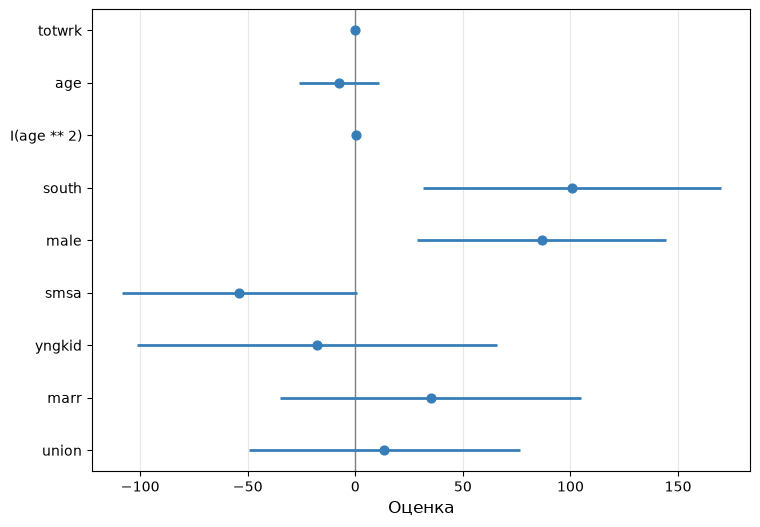
\includegraphics[keepaspectratio]{list08-ci_files/figure-pdf/fig-sleep-ci-output-1.png}}

}

\caption{\label{fig-sleep-ci}sleep equation \#2: 90\%-доверительные
интервалы для коэффициентов}

\end{figure}%

Почему интервалы для \texttt{totwrk} и \texttt{I(age\ **\ 2)} на рисунке
почти не видны? Значит ли это, что эти коэффициенты оценены точнее
остальных?

\begin{tcolorbox}[enhanced jigsaw, arc=.35mm, bottomrule=.15mm, bottomtitle=1mm, breakable, colback=white, colbacktitle=quarto-callout-tip-color!10!white, colframe=quarto-callout-tip-color-frame, coltitle=black, left=2mm, leftrule=.75mm, opacityback=0, opacitybacktitle=0.6, rightrule=.15mm, title=\textcolor{quarto-callout-tip-color}{\faLightbulb}\hspace{0.5em}{Ответ}, titlerule=0mm, toprule=.15mm, toptitle=1mm]

Нет: ширина интервала зависит от единиц измерения регрессора.
\texttt{totwrk} измерен в минутах в неделю, поэтому коэффициент и его
стандартная ошибка малы по величине. Чтобы сравнивать коэффициенты между
собой, их приводят к одному масштабу --- Рисунок~\ref{fig-sleep-ci-std}.

\end{tcolorbox}

Шкалированный коэффициент показывает, на сколько стандартных отклонений
меняется зависимая переменная при увеличении регрессора на одно
стандартное отклонение; значимость коэффициентов при шкалировании не
меняется.

\begin{figure}

\centering{

\pandocbounded{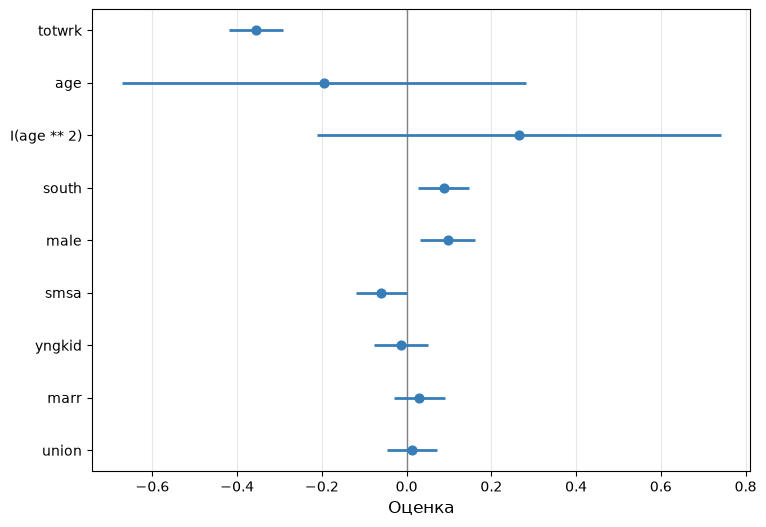
\includegraphics[keepaspectratio]{list08-ci_files/figure-pdf/fig-sleep-ci-std-output-1.png}}

}

\caption{\label{fig-sleep-ci-std}sleep equation \#2: 90\%-доверительные
интервалы для шкалированных коэффициентов}

\end{figure}%

\subsection{cost equation \#2}\label{cost-equation-2}

Для набора данных \texttt{Electricity} рассмотрим регрессию

\begin{verbatim}
np.log(cost) ~ np.log(q) + I(np.log(q)**2) + np.log(pl) + I(np.log(pl)**2) +
               np.log(pk) + I(np.log(pk)**2) + np.log(pf) + I(np.log(pf)**2)
\end{verbatim}

Ниже приведены 99\%-доверительные интервалы для коэффициентов.

\textbf{99\%-е доверительные интервалы (робастные стандартные ошибки,
HC3):}

{\def\LTcaptype{none} % do not increment counter
\begin{longtable}[]{@{}lrr@{}}
\toprule\noalign{}
Переменная & Нижняя граница & Верхняя граница \\
\midrule\noalign{}
\endhead
\bottomrule\noalign{}
\endlastfoot
Intercept & -129.940 & 41.133 \\
np.log(q) & 0.223 & 0.570 \\
I(np.log(q) ** 2) & 0.020 & 0.042 \\
np.log(pl) & -11.254 & 27.921 \\
I(np.log(pl) ** 2) & -1.544 & 0.633 \\
np.log(pk) & -3.795 & 4.668 \\
I(np.log(pk) ** 2) & -0.559 & 0.487 \\
np.log(pf) & -3.909 & 5.707 \\
I(np.log(pf) ** 2) & -0.734 & 0.673 \\
\end{longtable}
}

Модель была подогнана по 158 наблюдениям.

\begin{tcolorbox}[enhanced jigsaw, arc=.35mm, bottomrule=.15mm, bottomtitle=1mm, breakable, colback=white, colbacktitle=quarto-callout-important-color!10!white, colframe=quarto-callout-important-color-frame, coltitle=black, left=2mm, leftrule=.75mm, opacityback=0, opacitybacktitle=0.6, rightrule=.15mm, title=\textcolor{quarto-callout-important-color}{\faExclamation}\hspace{0.5em}{Условия теста}, titlerule=0mm, toprule=.15mm, toptitle=1mm]

\begin{itemize}
\tightlist
\item
  уровень значимости: \textbf{1\%}
\item
  стандартные ошибки: \textbf{робастные (HC3)}
\item
  гипотеза: \(H_0:\beta_j=0\) для каждого коэффициента, альтернатива
  двусторонняя
\end{itemize}

\end{tcolorbox}

Какие коэффициенты значимы?

Коэффициент значим на уровне 1\%, если 99\%-доверительный интервал не
содержит ноль.

\begin{tcolorbox}[enhanced jigsaw, arc=.35mm, bottomrule=.15mm, bottomtitle=1mm, breakable, colback=white, colbacktitle=quarto-callout-note-color!10!white, colframe=quarto-callout-note-color-frame, coltitle=black, left=2mm, leftrule=.75mm, opacityback=0, opacitybacktitle=0.6, rightrule=.15mm, title=\textcolor{quarto-callout-note-color}{\faInfo}\hspace{0.5em}{Коэффициенты, значимые на уровне 1\% (по робастным стандартным ошибкам
HC3)}, titlerule=0mm, toprule=.15mm, toptitle=1mm]

\texttt{np.log(q)}, \texttt{I(np.log(q)\ **\ 2)}

\end{tcolorbox}

На Рисунок~\ref{fig-cost-ci} интервалы показаны в исходных единицах
(константа не показана).

\begin{figure}

\centering{

\pandocbounded{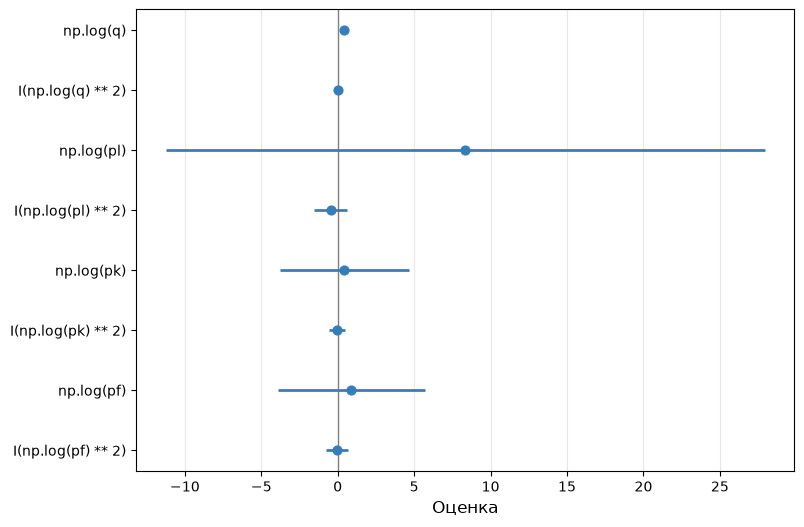
\includegraphics[keepaspectratio]{list08-ci_files/figure-pdf/fig-cost-ci-output-1.png}}

}

\caption{\label{fig-cost-ci}cost equation \#2: робастные
99\%-доверительные интервалы для коэффициентов}

\end{figure}%

Почему интервал для \texttt{np.log(pl)} намного шире остальных, а
интервалы для \texttt{np.log(q)} и \texttt{I(np.log(q)\ **\ 2)} почти не
видны?

\begin{tcolorbox}[enhanced jigsaw, arc=.35mm, bottomrule=.15mm, bottomtitle=1mm, breakable, colback=white, colbacktitle=quarto-callout-tip-color!10!white, colframe=quarto-callout-tip-color-frame, coltitle=black, left=2mm, leftrule=.75mm, opacityback=0, opacitybacktitle=0.6, rightrule=.15mm, title=\textcolor{quarto-callout-tip-color}{\faLightbulb}\hspace{0.5em}{Ответ}, titlerule=0mm, toprule=.15mm, toptitle=1mm]

Ширина интервала зависит от разброса регрессора: \texttt{np.log(pl)}
меняется в выборке мало (стандартное отклонение 0.17 против 1.81 у
\texttt{np.log(q)}). Кроме того, \texttt{np.log(pl)} и его квадрат почти
линейно зависимы, поэтому оба коэффициента оценены неточно. Чтобы
сравнивать коэффициенты между собой, их приводят к одному масштабу ---
Рисунок~\ref{fig-cost-ci-std}: интервал для \texttt{np.log(pl)} остаётся
самым широким.

\end{tcolorbox}

Шкалированный коэффициент показывает, на сколько стандартных отклонений
меняется зависимая переменная при увеличении регрессора на одно
стандартное отклонение; значимость коэффициентов при шкалировании не
меняется.

\begin{figure}

\centering{

\pandocbounded{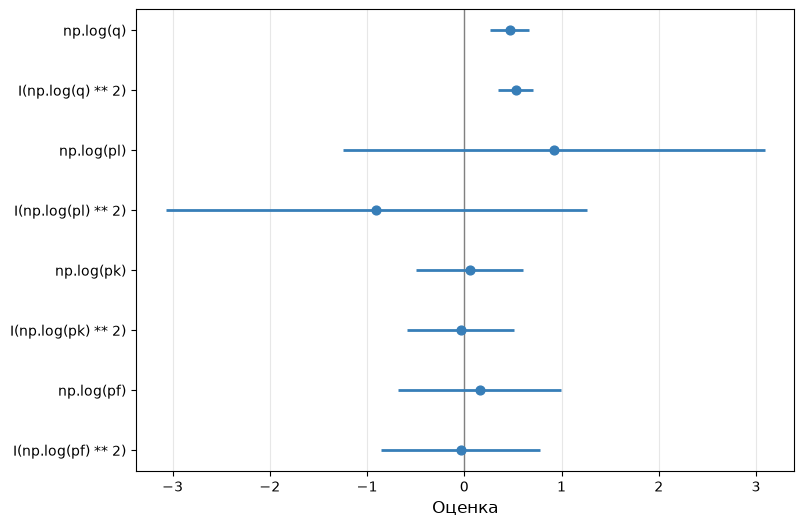
\includegraphics[keepaspectratio]{list08-ci_files/figure-pdf/fig-cost-ci-std-output-1.png}}

}

\caption{\label{fig-cost-ci-std}cost equation \#2: робастные
99\%-доверительные интервалы для шкалированных коэффициентов}

\end{figure}%

\section{Доверительные интервалы и сравнение
моделей}\label{ux434ux43eux432ux435ux440ux438ux442ux435ux43bux44cux43dux44bux435-ux438ux43dux442ux435ux440ux432ux430ux43bux44b-ux438-ux441ux440ux430ux432ux43dux435ux43dux438ux435-ux43cux43eux434ux435ux43bux435ux439}

\subsection{sleep equation \#3}\label{sleep-equation-3}

Для набора данных \texttt{sleep75} регрессия

\texttt{sleep\ \textasciitilde{}\ totwrk\ +\ age\ +\ I(age**2)\ +\ smsa\ +\ marr}

оценена по трём выборкам: Север (\texttt{south\ =\ 0}), Юг
(\texttt{south\ =\ 1}) и общая. В таблице --- оценки и стандартные
ошибки, на Рисунок~\ref{fig-models-ci} --- 95\%-доверительные интервалы.

{\def\LTcaptype{none} % do not increment counter
\begin{longtable}[]{@{}llll@{}}
\toprule\noalign{}
& Север & Юг & Общая \\
\midrule\noalign{}
\endhead
\bottomrule\noalign{}
\endlastfoot
Dep. Variable & sleep & sleep & sleep \\
totwrk & -0.159*** & -0.074 & -0.147*** \\
& (0.018) & (0.045) & (0.017) \\
age & -5.507 & -12.882 & -8.675 \\
& (12.557) & (25.039) & (11.271) \\
I(age ** 2) & 0.084 & 0.273 & 0.140 \\
& (0.150) & (0.299) & (0.135) \\
smsa & -59.812* & 16.055 & -69.924** \\
& (35.379) & (96.789) & (32.330) \\
marr & 28.034 & 152.296* & 47.598 \\
& (46.960) & (86.153) & (41.450) \\
Intercept & 3664.188*** & 3435.410*** & 3675.413*** \\
& (244.380) & (494.979) & (219.803) \\
R-squared & 0.129 & 0.140 & 0.118 \\
R-squared Adj. & 0.122 & 0.106 & 0.112 \\
F Statistic & 16.928*** & 4.043*** & 18.768*** \\
Observations & 576 & 130 & 706 \\
Residual Std. Error & 421.078 & 393.300 & 418.809 \\
\end{longtable}
}

\emph{Signif. codes:} \texttt{***} \(p<0.01\), \texttt{**} \(p<0.05\),
\texttt{*} \(p<0.1\). В скобках --- неробастные стандартные ошибки.

\begin{figure}

\centering{

\pandocbounded{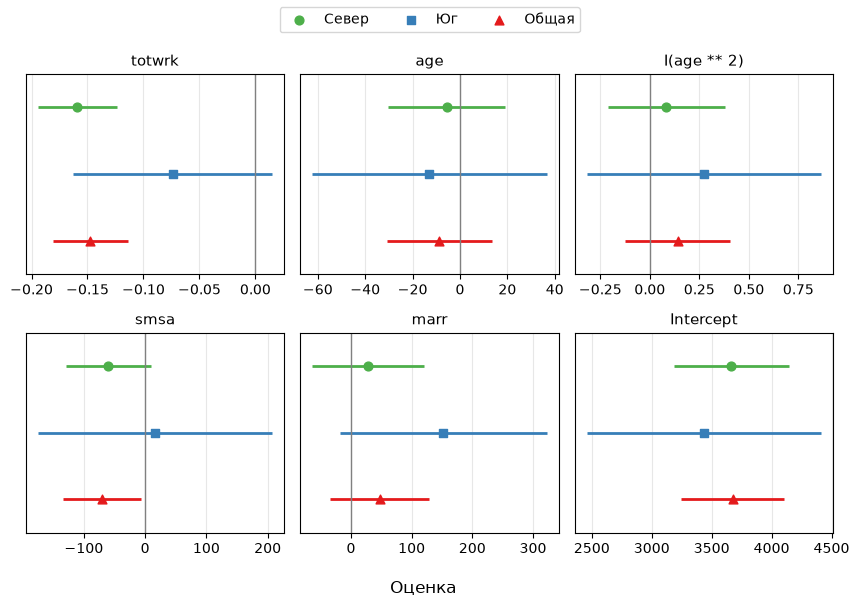
\includegraphics[keepaspectratio]{list08-ci_files/figure-pdf/fig-models-ci-output-1.png}}

}

\caption{\label{fig-models-ci}sleep equation \#3: 95\%-доверительные
интервалы для коэффициентов трёх моделей (неробастные стандартные
ошибки)}

\end{figure}%

\begin{enumerate}
\def\labelenumi{\arabic{enumi}.}
\tightlist
\item
  Для каких коэффициентов 95\%-доверительные интервалы моделей «Север» и
  «Юг» не пересекаются?
\item
  Можно ли по пересечению интервалов сделать вывод, что коэффициенты в
  двух подвыборках одинаковы? Каким тестом проверяется эта гипотеза?
\end{enumerate}

\begin{tcolorbox}[enhanced jigsaw, arc=.35mm, bottomrule=.15mm, bottomtitle=1mm, breakable, colback=white, colbacktitle=quarto-callout-tip-color!10!white, colframe=quarto-callout-tip-color-frame, coltitle=black, left=2mm, leftrule=.75mm, opacityback=0, opacitybacktitle=0.6, rightrule=.15mm, title=\textcolor{quarto-callout-tip-color}{\faLightbulb}\hspace{0.5em}{Ответ}, titlerule=0mm, toprule=.15mm, toptitle=1mm]

Интервалы пересекаются для всех коэффициентов. Пересечение интервалов не
является тестом равенства коэффициентов; гипотеза об отсутствии
структурных сдвигов проверяется F-тестом (тест Чоу), см. листок
list07-F-test.

\end{tcolorbox}




\end{document}
